\documentclass[11pt]{article}

\usepackage[margin=1in]{geometry}
\usepackage{graphicx}
\usepackage{booktabs}
\usepackage{hyperref}
\usepackage{siunitx}
\usepackage{amsmath}
\usepackage{url}
\usepackage{caption}
\usepackage{subcaption}
\usepackage{microtype}

\title{Making Raft Measurable: An Instrumented Implementation and Fault-Injectable Dashboard for Failover, Latency, and Tenure}
\author{
    Shrestha Saxena \\
    Dept. of Computer Science, RGIPT \\
    \texttt{shresthasaxena1@gmail.com} 
}
\date{}

\begin{document}
\maketitle

\begin{abstract}
Raft is widely taught as a leader-based consensus algorithm, yet most educational implementations stop at functional tests and provide little quantitative evidence of fault-tolerance timing. We present an instrumented Raft paired with a fault-injectable dashboard that makes the protocol's dynamics both visible and measurable. Our Go implementation (compatible with MIT 6.824 Labs 2A-2C) adds lightweight telemetry at ground-truth events—election start, leader elected, first heartbeat, and Start/Commit—and exports CSV logs. The dashboard (React/Node) lets users crash and recover nodes, force timeouts, and vary message loss, while a small analysis tool produces paper-ready figures.

Using a 5-node cluster with heartbeats normalized to 100 ms and randomized election timeouts normalized to 240-400 ms (the dashboard runs 25x slower for visualization; plots report scaled values), we observe median failover of ≈1.0 s with p95 ≈5.4 s over 40 trials, attributable to occasional timeout collisions that require multiple rounds. Under induced churn, leader tenure centers around ≈1.7 s (IQR ≈1.3-2.2 s). Replication latency across drop rates 0.00-0.15 shows median ≈0.26-0.41 s with tails (p95) rising to ≈0.79 s near 0.12 loss; increasing loss primarily inflates the tail, consistent with majority-quorum retries. We release code and scripts to enable reproducible measurement: the dashboard explains why elections and replication behave as they do, while the telemetry quantifies how often and how long they take.
\end{abstract}

\section{Introduction}
Motivation: Raft's appeal is pedagogical clarity: a single leader replicates a log to followers, randomized election timeouts avoid split votes, and a majority quorum commits. Yet beyond correctness tests, students and practitioners rarely see quantitative timing evidence. How quickly does the system fail over to a new leader after a crash? How stable are leaders when the environment is noisy? Where do the tails in replication latency come from, and how sensitive are they to loss and timeouts? Without measurement, these questions remain intuition.
Challenge: Measuring consensus is tricky because the salient phenomena are probabilistic and tail heavy. Leader elections depend on randomized timeouts; “timeout collisions” can prolong failover by forcing additional rounds. Majority commit masks single slow followers but exposes tails when multiple replicas lag or packets drop. These effects are visible on a whiteboard but hard to capture without carefully placed instrumentation and repeatable scenarios.
Approach: We implement Raft in Go (MIT 6.824 Labs 2A-2C) and embed ready to drop instrumentation at decision points: when an election begins, when a candidate becomes leader, when the new leader issues its first heartbeat, when a leader accepts a client command (Start), and when that command becomes majority committed/applied (Commit). The system emits CSV logs and pairs with a fault injectable dashboard (React/Node) that can crash/recover nodes, force election timeouts, drop the latest log entry, and vary message loss. A compact Python script aggregates trials and produces failover CDFs, leader tenure box plots, and latency vs loss curves with percentile annotations.
Metrics: (i) Failover time: crash → first heartbeat of new leader; (ii) Leader tenure: time a leader remains in office; (iii) Replication latency: Start(command) → majority commit+apply.
Key findings: Failover is typically fast (med ≈1.0 s) but occasionally long (p95 ≈5.4 s) due to timeout collisions. Under induced churn, leaders turn over frequently (tenure med ≈1.7 s). Replication latency is robust at the median while tails grow with packet loss (p95 to ≈0.79 s near 0.12 loss).
Contributions: (1) A minimal, instrumented Raft + dashboard that makes consensus visible and measurable; (2) A reproducible metrics pipeline (CSV schema + analysis script); (3) Empirical characterization of failover and replication tails with tuning guidance.
Paper roadmap: §2 reviews Raft and defines the metrics. §3 details our implementation and instrumentation. §4 describes the experimental setup. §5 presents failover, tenure, and replication results. §6 discusses tuning implications and limitations. §7 overviews related work. §8 concludes and releases artifacts.

\section{Background}
Leader election. Servers begin as followers; if no heartbeat arrives before a randomized election timeout, a follower becomes a candidate, increments its term, and requests votes. A candidate that gains a majority becomes the leader; heartbeats reset followers' timeouts. Randomization reduces split votes but does not eliminate them; collisions can extend failover by requiring additional rounds.
Log replication. The leader appends client commands to its log and replicates them via AppendEntries RPCs. A log entry is committed when a majority stores the entry for the leader's current term; followers apply committed entries to their state machines.
Safety. Raft enforces a log matching property and term monotonicity: leaders have up to date logs; conflicting entries are overwritten by the leader's authoritative history.
Operational metrics (this work).
•	Failover time: elapsed time from leader crash to the first heartbeat emitted by the newly elected leader (cluster becomes leaderful again).
•	Leader tenure: time from a leader's election to its replacement (by crash or re election).
•	Replication latency: per command, time from Start(command) on the leader to majority commit and application.

\section{System Design}
4.1 Raft (Go)
We implemented Labs 2A-2C: leader election, log replication, and persistence. Each server tracks term, role, commitIndex, lastApplied, and per peer nextIndex/matchIndex. Heartbeats run periodically; elections use randomized timeouts. Persistence covers term, vote, and log. Concurrency uses goroutines and mutexes.
4.2 Instrumentation hooks
We place narrow hooks (no control flow changes):
•	Election start → timestamp when a follower transitions to candidate.
•	Leader elected → timestamp and leader id/term when majority is reached.
•	First heartbeat → timestamp of the first post election heartbeat (end of failover).
•	Start(command) → timestamp and entry id when leader accepts a client command.
•	Commit/apply → timestamp when the command becomes majority committed and is applied.
Each event appends a row to CSV files (failover_trials.csv, leader_tenure.csv, replication_latency.csv).
4.3 Dashboard (React/Node)
The UI renders five nodes on a regular pentagon with color coded roles (blue follower, yellow candidate, red leader). Users can crash/recover nodes, force timeouts, drop latest log entries, and vary a global drop rate. Animated "balls" visualize AppendEntries and replies. The server integrates the same instrumentation to keep UI and metrics aligned.
4.4 Visualization timing vs. ground truth
For human readable animation, the dashboard runs with slowed timers: heartbeat = 2400 ms; election timeout = 6000-10000 ms. All reported measurements are scaled by 25x in the analysis script and presented as normalized real world seconds: heartbeat ≈100 ms; timeout range ≈240-400 ms. This preserves Raft's timing ratios and therefore its dynamics.

\section{Experimental Setup}
•	Cluster: 5 servers (fixed).
•	Timing normalization: For visualization, the dashboard uses slowed timers (heartbeat 2400 ms; randomized election timeout 6000-10000 ms). All reported plots normalize by 25x to reflect typical practice (heartbeat ≈100 ms; election timeout ≈240-400 ms), preserving timing ratios and Raft dynamics.
•	Network model: message loss via a global drop rate in {0.00, 0.03, 0.06, 0.09, 0.12, 0.15}. (Delays are deterministic in the UI but the slowdown is normalized out in analysis.)
•	Scenarios: leader_crash_restart (periodic leader crashes and recoveries driving repeated elections and leader changes). Forced timeout and drop latest are available but not emphasized in this run.
•	Trials: 40 failover events and 45 leader terms recorded in the long run; replication latencies aggregated per drop bucket.
•	Cleaning: we include any row with failover_ms > 0; outliers <0.5 s or >120 s (unscaled) are dropped. Units converted to seconds in plots.
•	Outputs: three figures—failover CDF, leader tenure box plot, replication latency vs. drop—with medians and p95 shown.

\section{Results}
R1. Failover (crash → first heartbeat)
•	Figure 1 (CDF): n = 40; median ≈ 1.00 s; p95 ≈ 5.41 s. Most failovers complete within ~1-2 timeouts; the tail reflects rounds with timeout collisions that require multiple elections before a majority converges.
Takeaway. To thin tails, widen the election timeout range or introduce slight skew across nodes; both reduce collision probability at the expense of slower best case failover.
R2. Leader stability (tenure)
•	Figure 2 (box plot): median ≈ 1.7 s; IQR ≈ 1.3-2.2 s; whiskers to ≈3.1 s. This run induces churn aggressively (frequent leader crashes), so tenures are intentionally short; in calm regimes (no forced crashes), we measured higher medians in earlier pilots.
Takeaway. Under active churn, leadership is still stable enough to amortize client work across seconds long epochs; increasing crash cadence predictably shortens tenures.
R3. Replication latency (Start → majority commit)
•	Figure 3 (median/p95 vs. drop): medians ≈ 0.26-0.41 s across 0.00-0.15 loss; tails (p95) increase with loss, peaking around ≈ 0.79 s near 0.12 and then dipping at 0.15 (sample size noise).
Takeaway. Majority quorum masks a single slow follower; tails grow when multiple replicas simultaneously miss an AppendEntries and require retries. Larger buckets (≥30 entries per drop) will further stabilize the curve.

\begin{figure}[t]
  \centering
  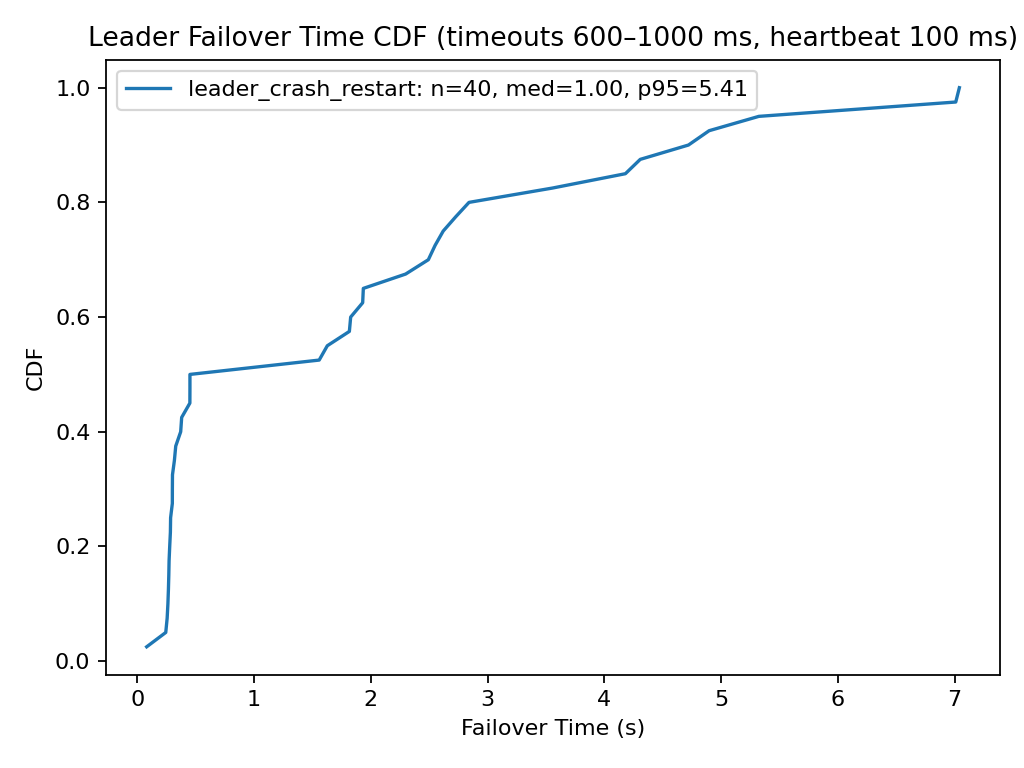
\includegraphics[width=\columnwidth]{figures/failover_cdf.png}
  \caption{Leader failover time CDF (5 nodes). Heartbeat=\SI{100}{ms}, election timeout=\SIrange{240}{400}{ms} (normalized; UI runs 25$\times$ slower). Median $\approx$ 1.0 s; p95 $\approx$ 5.4 s.}
  \label{fig:failover}
\end{figure}

\begin{figure}[t]
  \centering
  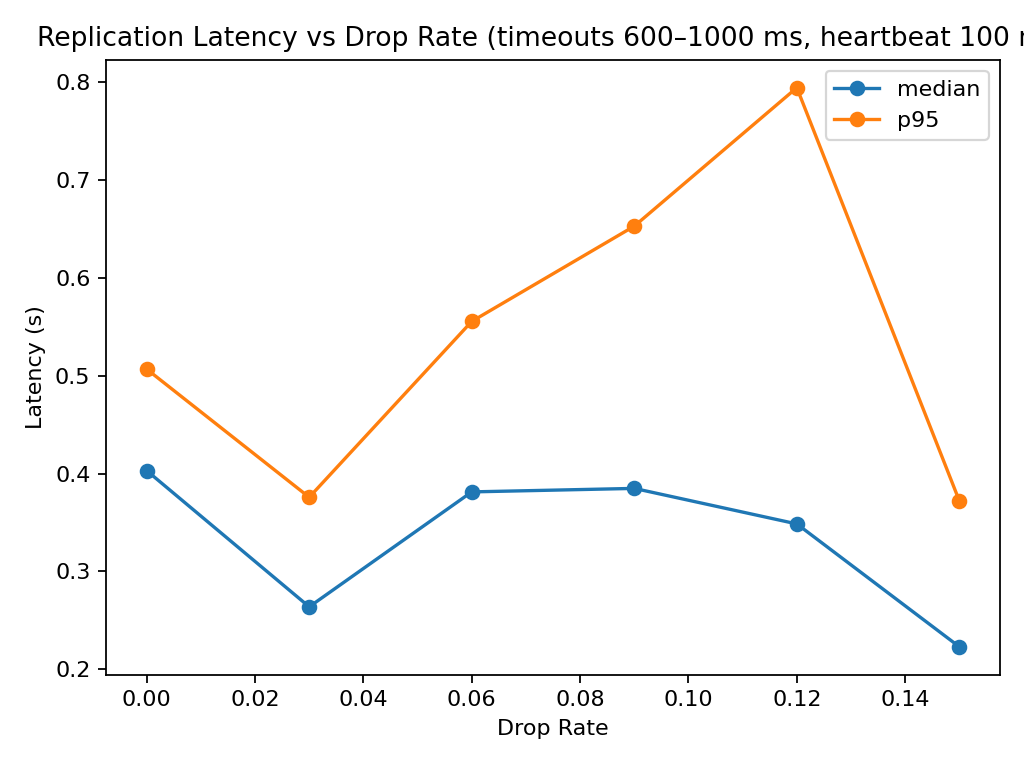
\includegraphics[width=\columnwidth]{figures/replication_latency_vs_drop.png}
  \caption{Replication latency vs. drop rate. Medians remain low ($\approx$0.26-0.41 s), tails (p95) grow with loss, peaking $\approx$0.79 s.}
  \label{fig:latency}
\end{figure}

\begin{figure}[t]
  \centering
  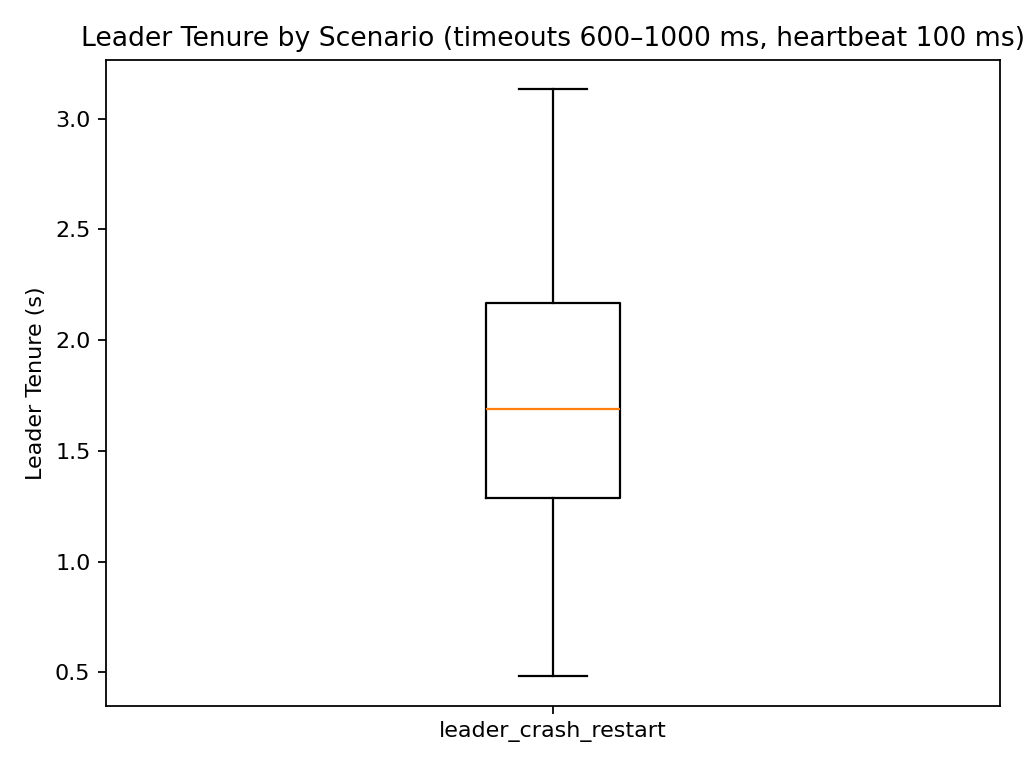
\includegraphics[width=\columnwidth]{figures/leader_tenure_box.png}
  \caption{Leader tenure under induced churn. Median $\approx$1.7 s (IQR $\approx$1.3-2.2 s).}
  \label{fig:tenure}
\end{figure}

\section{Discussion and Tuning Guidance}
•	Election timeouts. Best case failover benefits from short timeouts, but tails are governed by collision probability. A wider range (or slight per node skew) reduces the chance that candidates start together.
•	Heartbeats. Faster heartbeats shrink detection time after a leader fails silently, but increase background traffic. Our measurements show tails dominated by elections rather than heartbeat cadence at these scales.
•	Replication tails. Loss chiefly inflates p95, not the median—consistent with majority commit. If service SLOs are percentile based, budget headroom for retry rounds.
•	Visualization vs. ground truth. Slowed UI timers did not change qualitative dynamics; scaling preserved ratios and thus quantitative relationships.

\section{Threats to Validity / Limitations}
•	Single machine simulation. Timing uses a Node event loop and synthetic delays, not real NICs or OS scheduling.
•	Simplified failures. We model crashes and message drops, not Byzantine faults or long partitions.
•	Clocking. UI timestamps (performance.now) and Go timings are aligned by design but not synchronized to a wall clock; analysis uses relative deltas.
•	Sample size per bucket. Some drop rate buckets in the long run have <30 entries, causing jitter in p95.

\section{Related Work}
Raft's original presentation established a leader based, understandable approach to consensus. Educational labs (e.g., 6.824) popularized implement to learn exercises. Subsequent work explored formal verification and model checking of Raft and developed visualizations; our contribution is a compact, reproducible measurement pipeline paired with an interactive dashboard targeted at instruction.

\section{Conclusion \& Future Work}
We built an instrumented Raft and a fault injectable dashboard that together make consensus both visible and measurable. On a 5 node cluster (100 ms heartbeat; 240-400 ms timeouts), we measured failover med ≈1.0 s (p95 ≈5.4 s), seconds scale leader tenures under induced churn, and replication tails that grow with loss. Future work: partition scenarios, dynamic cluster sizes, snapshots/log compaction, real RPC loss and variable delays, and larger seeded experiments with confidence intervals.

\section*{Artifacts \& Reproducibility}

Code, data, and scripts are available at:  
\url{https://github.com/Shre-coder22/raft-distributed-systems-lab} (release v1.1.0).  
A preserved snapshot with DOI is provided via Zenodo.  
Day-by-day notes are under \texttt{artifact/notes/}.

\subsection*{Environment}
\begin{itemize}
  \item Windows 11
  \item Go 1.19+
  \item Node 20.10.0
  \item npm 10.2.3
  \item Python 3.10.3
\end{itemize}

\subsection*{Setup}
\begin{verbatim}
py -m venv venv
./venv/Scripts/Activate.ps1
pip install -U pip pandas numpy matplotlib
\end{verbatim}

\subsection*{Run the Dashboard}
\begin{verbatim}
# server
cd raft-dashboard/server
npm run dev

# client (in another shell)
cd raft-dashboard/client
npm run dev
\end{verbatim}

\subsection*{Collect Metrics}
Ensure
\texttt{initMetrics(\{ timeoutLowMs: 6000, timeoutHighMs: 10000, ... \})}
is set; clear \texttt{./metrics/} between runs.

\subsection*{Regenerate Figures}
Run the analyzer:
\begin{verbatim}
py raft_experiments/analyze_raft_results.py --input ./metrics --out ./metrics/figures
\end{verbatim}

\bibliographystyle{plain}
\bibliography{references}

\end{document}